\documentclass[10pt]{beamer}
\usetheme{fibeamer}
\setbeamertemplate{itemize item}{\tiny\raise1.6pt\hbox{$\bullet$}}

\usepackage{lmodern}
\usepackage{xcolor}
\usepackage{wrapfig}
\usepackage[font=small,skip=0pt]{caption}
\definecolor{GGrey}{HTML}{232323}



\title{Laboratory on Neural Networks}
\subtitle{TensorFlow}
\author{Luca Erculiani}
\institute{University of Trento}
\date{}

\begin{document}
\def \bgcc {gray!20!white} 

\maketitle

%-----------------------------------------------------------------------------%

\defverbatim[colored]\localrun{
\begin{lstlisting}[language=bash,backgroundcolor = \color{\bgcc}]
> ./jupyter-scikit.sh
\end{lstlisting}}
\begin{frame}{Setup}
\centering


\includegraphics[width=0.4\textwidth]{figures/colab}

\vspace{0.3in}
Download and extract the lecture material from:

{\footnotesize \scriptsize \url{http://disi.unitn.it/~passerini/teaching/2019-2020/MachineLearning/}}

\vspace{0.2in}
Open Google colab on your web browser and login (with your unitn account or a personal one): \\

{\url{https://colab.research.google.com}} \\

\end{frame}

%-----------------------------------------------------------------------------%

\defverbatim[colored]\pipinstall{
\begin{lstlisting}[language=bash,backgroundcolor = \color{\bgcc}]
> pip install numpy scipy matplotlib sklearn jupyter
\end{lstlisting}}

\defverbatim[colored]\launchjupyter{
\begin{lstlisting}[language=bash,backgroundcolor = \color{\bgcc}]
> jupyter notebook
\end{lstlisting}}

\begin{frame}{Setup}
\centering

Upload the file \texttt{tensorflow-lab.ipynb} \\
\vspace{0.2in}

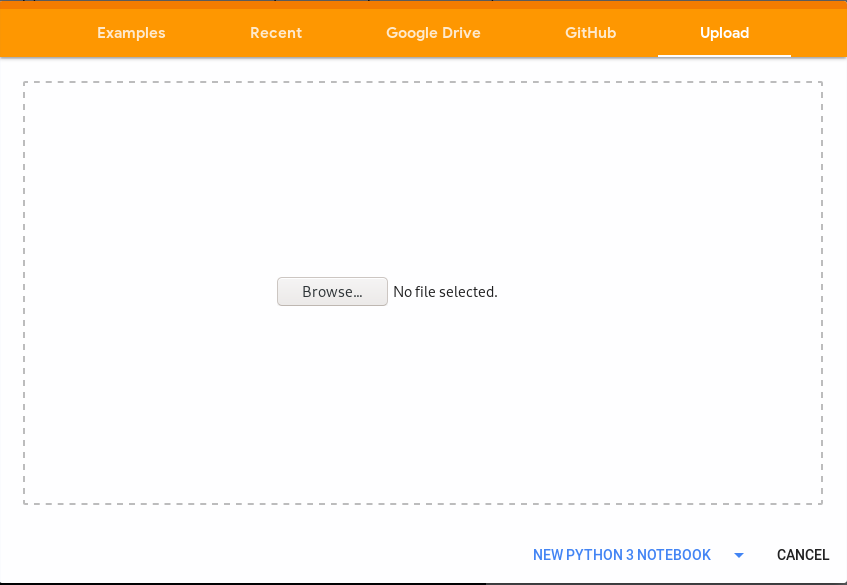
\includegraphics[width=0.75\textwidth]{figures/upload}

\end{frame}

%-----------------------------------------------------------------------------%


%-----------------------------------------------------------------------------%

\begin{frame}{Assignment}
\centering

For the third Machine Learning assignment you will solve a classification task
using \textbf{TensorFlow} over the OCR dataset. The dataset is already split
into training and test sets. Your task is to train a deep
neural network with {\bf at least 3} convolutional layers on the training set and predict the labels on the test set. To
pass the assignment, your network has to classify the examples in the test
set with higher accuracy than the reference baseline for the dataset.

		Additionally, you need to perform \textbf{model selection}  
		(optimize at least one hyperparameter) and 
test your algorithm over a validation set
and produce a report containing the results obtained.


\end{frame}

%-----------------------------------------------------------------------------%

\begin{frame}{Assignment | Material}

Download the assignment material:

{\footnotesize \url{http://disi.unitn.it/~passerini/teaching/2019-2020/MachineLearning/}}

The material contains:
    \begin{itemize}
    \item The training set examples;
    \item The training set labels;
    \item The test set examples;
    \item The test set labels;
    \item A README containing info about the dataset. \\ this file also contains
          the reference baseline accuracy;
    \end{itemize}

\end{frame}

%-----------------------------------------------------------------------------%

%\begin{frame}{Assignment | Helper}
%
%The helper script can be used to test your predictions. Given a file containing
%the predicted labels, the helper script sends the labels to our server and
%receives the prediction accuracy. You can use it in this way:
%
%\mint[fontsize=\scriptsize, bgcolor=GGrey]{cucumber}| >> ./helper.py your.email test-labels.txt |
%
%\vspace{-0.3in}
%The first parameter is your \texttt{unitn} email, the second parameter is the
%path to the file containing the predicted labels. This file should contain one
%label per line in the same order of the file containing the examples. The labels
%should be in the same format of the labels in the training set.
%
%The helper also prints the current best accuracy achieved by any of you on that
%dataset, just to put a bit of healthy competition! :)
%
%\end{frame}

%-----------------------------------------------------------------------------%

\begin{frame}{Assignment}
\framesubtitle{Step-by-step}


\begin{enumerate}
		\item Build a neural network (at least 3 convolutional layers);
\item {\bf Do model selection} (optimizing hyperparameters
		or testing different architectures, performing validation by splitting the train set);
\item Train your network over the full training set;
\item Use the network to predict the examples in the test set;
\item Place the labels in a file, in the same order as you read the test
      examples and in the same format of the labels in the training set.
\end{enumerate}

\end{frame}

\begin{frame}{Assignment}
\framesubtitle{Report}

 Write a report describing the learning algorithm used and discussing the
results obtained; The report should contain at least:
    \begin{itemize}
    \item The average accuracy over the your validation set and over the test set.
    \item A simple diagram of the network architecture (use Google Drawings or similar software);
	\item For each layer:  number of weights, their shape, and the shape of the output.
    \end{itemize}

\end{frame}
%-----------------------------------------------------------------------------%

\begin{frame}{Assignment}
\framesubtitle{Submit}

\begin{itemize}
    \item After completing the assignment submit it via email
    \item Send an email to \href{mailto:mllab@unitn.it}{mllab@unitn.it} 
    \item Subject: tensorflowSubmit2019
    \item Attachment: \texttt{id\_name\_surname.zip} containing:
    \begin{itemize}
        \item The text file containing the final predictions;
        \item The code you used;
        \item The report in PDF format.
    \end{itemize}
\end{itemize}
\begin{alertblock}{NOTE}
    \begin{itemize}
	\item \textbf{No group work}
        \item This assignment is mandatory in order to enroll to the oral exam
    \end{itemize}
\end{alertblock}

\end{frame}

%-----------------------------------------------------------------------------%

\end{document}
